\section{Overview Internet of Things and Related Concepts }
\subsection{Internet of Things}
The concept of Internet of Things was first coined by Kevin Ashton, Executive Director of the Auto-ID Center in Massachute Institute of Technology (MIT) in 1999, and it is described as a world where billions of objects can sense, communicate and share information \cite{madakam2015internet}. Then IoT becomes more popular due to the explosion of mobile devices, ubiquitous communication, cloud computing. However, the definition of ``Internet of Things'' is still ambiguous, and have different facets depending on the perspective. From the view of functionality and identity, IoT is defined as ``Things having identities and virtual personalities operating in smart space using intelligent interfaces to connect and communicate within the social, environmental, and user contexts'' \cite{ray2018survey}. Semantically, the term of Internet of Things is composed of two words ``Internet'' and ``Things''. Following this way, IoT could be defined as ``a worldwide network of interconnected object uniquely addressable, based on standard communication protocols''~\cite{minerva2015towards}.\\

Similar to its definition, the characteristic of IoT vary from one domain to another. Some of the key characteristics identified during the research study are as follows:
\begin{itemize}
    \item \textbf{Dynamic and Self-adapting}: IoT devices and system must be able to dynamically adapt with the changing contexts or sensed environment. For example: considering a smart building system comprising of a number of temperature devices. These devices can adapt their modes based on whether it is indoor or outdoor. Based on that, they can adjust the calibrations to collect data more accurately. In this example, the smart building system is adapting itself with the change of context or environment.
    
    \item \textbf{Self-configuring}: IoT device may have the capability to configure themselves relating connection, software upgrades, etc., while minimal user intervention.  This characteristic allows co-operating a large number of devices to provide specific functionality.
    
    \item \textbf{Interoperable Communication Protocols}: The IoT devices may support multiple connectivity (Wifi, Lora, Sigfox, etc.) to communicate with other devices as well as the cloud infrastructure.
    
    \item \textbf{Unique Identify}: IoT device must be identified by a unique identity (such as an IP address or an URL). In addition, the IoT system needs to provide intelligent interface allowing the end-user to access directly these devices.
    
    \item \textbf{Integrated into Information Network}: In order to communicate and exchange data, IoT devices are integrated into the information network. In addition, these devices can be dynamically described and discovered in the network by other IoT devices or systems. For example A weather station can describe its monitoring information to other station in the same information network so that they can communicate and exchange collected data. Such integration could enrich the acquired information because of the data aggregation from several nodes.
    
\end{itemize}

\subsection{Web of Things and Semantic Web of Things}
Recent years, we have been witnessing the explosion of Internet of Things in term of the number and types of IoT devices. Unfortunately, there is no universal application protocol that is compatible with various networking interface. Thus, building a single global ecosystem of Things communicating with each other seamlessly is still impossible~\cite{WebofThi19:online}. In other words, the IoT is a collection of ``Silos of Things'' that can not interact with each other. Therefore, to build a global Internet of Things, we need a universal language and protocols supporting the interaction between devices and application regardless their properties (types, firmware, configuration, etc.). Instead of inventing a dedicated technology, leveraging the widely popular web protocols, standards, and blueprints to make data and services offered by Things more accessible to a larger pool of developer~\cite{guinard2016building}. That is premise behind adoption of the Web of Things. The ultimate goal of Web of things is effectively breaking the ``Silos of Things'' also known as ``one device, one protocol, one app'' by applying tools and techniques that are available on the Web technology.

In order to archive its goals, WoT is used on the Application level to abstract the complexity and variety of lower-level (protocols, firmware, data formats, etc.) by a simple Web model to facilitate the integration of all IoT devices and application. In other words, by hiding the heterogeneity of IoT devices and application behind Web technologies, the WoT allows developers to focus on their application without considering the technologies behind. In practice, the developers could interact with IoT Things via web browsers and explore the Things as surfing the web. The collected data from Things is visually displayed using Web programming language such as HTML, CSS, and Javascript. 

In general, the Web of Things facilitates the interaction and exchange of information between different Things and System powered by Web technologies. However, the exchanged data can be encoded and presented under different formats (envelopes, semantics, and meta-data) . For example, the collected data presenting current temperature can be under plain text, XML/EXI, or JSON format. The file name can be ``temperature'' or ``temp''. Therefore, it is necessary to build a Semantic Web of Things (SWoT) to ensure a common understanding and format. In other words, SWoT concept is the evolution of the Web on Things with the Semantic technology. The goal of SWoT is to provide comprehensive interoperability that allows not only sharing and reuse of IoT Things but also making IoT data to be universally understandable~\cite{pfisterer2011spitfire}. The summary of evolution from Internet of Things to Web of Things is illustrated in Figure~\ref{fig:c2_evolution_iot_swot}

\begin{figure}[h!] 
 \begin{center} 
 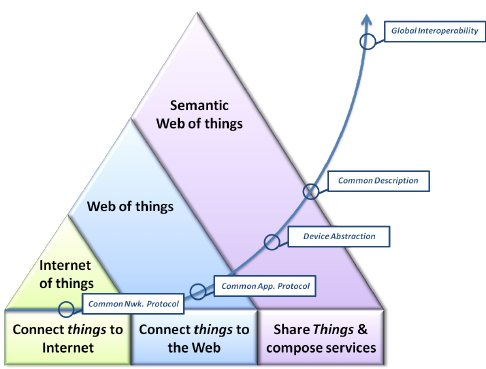
\includegraphics[width=0.72\textwidth]{./Part1/Chapter2/figures/c3_evolution_iot_swot.jpg} 
    \caption{Evolution of the solutions for multicast mobility.~\cite{jara2014semantic}}
     \label{fig:c2_evolution_iot_swot}
  \end{center} 
\end{figure}

\subsection{Massive Internet of Things}
With the explosion of Internet of Things, the number of Things and its connectivity have been growing exponentially. In addition, Things is no longer just send the data to cloud, but also exchange information to each other. As a result, Massive IoT is emerging as a new focal point for IoT connectivity technologies referring to huge volume of constrained IoT devices, which stringently require excellent coverage, cost-effective and low-energy consumption~\cite{Northstream2017}. Among several new connectivity technologies for MIoT, proprietary LPWAN technologies such as Sigfox and LoRA have been considering the most potential candidates while cellular-based connectives such as 5G or NB-IoT are under developing and testing process \cite{raza2017low}.

On a technical level, the IoT devices in Massive Internet of Things context are distributed in a wide area from large manufacturing plants to inside sewer systems where the radio signal is physically challenging. To adapt to such environments, the connectivity technology of Massive IoT is not only wide coverage but also robust. In addition, replacing device battery in large area is very expensive. This connectivity technology must be low energy consumption to extend the device battery life. Typically, high throughput and latency are not unessential in massive IoT applications, since they more focus on collecting data than controlling.


\section{Fundamentals of IoT}
\subsection{IoT Things}
Similar to Internet of Things definition, deriving a unified definition for the ``Things’’ in IoT is still challenging although it has received most attention from academic organizations such as NIST, ITU, W3C, IERC, and IETF~\cite{Liu2016}. IEEE simply defined the Things as a physical object that is relevant from a user or application perspective~\cite{minerva2015towards}. However, IERC believes that a Thing can be physical or virtual and identified by unique identity~\cite{smith2012internet}. NIST proposes the Things can be all software, all hardware, or the combination of software and hardware.~\cite{voas2016networks}. 

Due to the heterogeneity in Things definition, we simplify the Thing could be physical or virtual object integrated into a network. This object can interact via a unique identity and intelligent interface. For example, a smart phone can be a Thing which is physical object, able to join networks (WiFi, cellular network), has unique identity (phone number, IP address) and intelligent interface. A database is also considered as a Thing because it is a virtual object, able to join networks (internet), has unique identity (URL) and intelligent interface (Web services).
\subsection{IoT Connectivity}
In this section, rather than mentioning all the IoT protocol following existing architecture model like OSI models, we only present some dedicated protocols in IoT and organize them based on their functionality.

\begin{description}
\item[\textbf{Infrastructure}:\\]
    \begin{itemize}
    \item[] 
    \item \textit{6LoWPAN: } This is an acronym of IPv6 over Low Power Wireless Personal Area Networks defined by the Internet Engineering Task Force, IETF in their document RFC 6282~\cite{shelby20116lowpan} deriving from the idea that "the Internet Protocol could and should be applied even to the smallest devices,"~\cite{Mulligan:2007:ARC:1278972.1278992}. This protocol uses 2.4 GHz frequency with 250 kbps rate.
    
    \item \textit{uIP: } The uIP is an open source project licensed under a BDS style license~\cite{adamdunk86:online}. The goal of this project is to create a dedicated TCP/IP stack for 8 or 16 bits micro-controllers. Currently, it is further developed by wide community.
    
    \item \textit{NanoIP: } The concept NanoIP is to optimize all features of Internet to adapt to embedded and small devices, without the overhead of TCP/IP~\cite{shelby2003nanoip}.NanoIP uses two dedicated transport techniques are nanoUPD and nanoTCP. A socket-compatible API is also provided to make sure the protocol similar to original IP protocol.
    
    \item \textit{Time Synchronized Mesh Protocol (TSMP): } TSMP is a communication protocol designed for self-origanizing network of wireless devices enabling reliable, low power, secure communication~\cite{pister2008tsmp} 
    
    \end{itemize}

\item[\textbf{Discovery}:\\]
    \begin{itemize}
    \item[] 
    \item \textit{mDNS: } The mDNS is used to resolves host names to IP addresses within small networks. Except do not include a local name server,  this technology is essentially the same with the unicast Domain Name System (DNS) in term of programming interfaces, packet formats and operation~\cite{cheshire2013multicast}. 
    \item \textit{Physical Web: } The Physical Web aims to discover and interact with nearby devices through a list of URLs being broadcast. That means every smart object in the network needs to broadcast its access URL that any nearby device can receive. 
    \item \textit{HyperCat: } HyperCat is an open, lightweight JSON-based hypermedia catalogue format to exploit Thing resources~\cite{HyperCat76:online}. It allows adding a set of semantic annotations to Things resources and make them discoverable over the web. 
    \item \textit{Universal Plug and Play (UPnP): } The UPnP uses Internet and Web protocols to automatically discover new devices to be plugged into a network. These new devices announce their presence to other devices by using a discovery protocol based on HTTP~\cite{RFC6970U68:online}. 
    
    
    \end{itemize}

\item[\textbf{Data Protocol}:\\]
    \begin{itemize}
    \item[] 
    \item \textit{Message Queuing Telemetry Transport (MQTT): } MQTT \index{MQTT} is an publish-subscribe based messaging protocol working on the top of TCP/IP protocol. It is useful for connections limited bandwidth~\cite{}. An MQTT system consist of a central messaging server named "message broker" and clients. There are two client types are: (1) publisher: clients publish data to broker. (2) Subscriber: Clients receive data from broker. The responsibility of broker is to forward data from publishers to subscribers. 
    
    \item \textit{Constrained Application Protocol (CoAP): } CoAP \index{CoAP} is an application layer protocol designed for constrained internet devices that are limited in storage, computation power. It is based on RESTful protocol design to simply translate to HTTP for simplified integration, while also meeting specialized requirements such as multicast support, very low overhead, and simplicity~\cite{RFC7252T93:online}. Currently, the major standardization for CoAP is done by The Internet Engineering Task Force (IETF) and various new functionalities have been added~\cite{colitti2011integrating}. 
    
    \item \textit{Extensible Messaging and Presence Protocol (XMPP): } XMPP \index{XMPP} is a real-time communication protocol based n Extensible Markup Language (XML). It is defined in an open standard managed by The Internet Engineering Task Force (IETF). Dsigned to be extensible, the protocol is also used for publish-subscribe model in VoIP~\index{VoIP}, video and IoT application \index{IoT!application}. 
    
    \item \textit{Advanced Message Queuing Protocol (AMQP): } Similar to XMPP\index{XMPP}, AMQP is an open standard application layer but it is designed for message-oriented middleware. Thereby, its functionalities ensure reliability and security such as message orientation, queuing, routing~\cite{o2007toward}. The authentication and encryotion based on Simple Authentication and Security Layer(SASL)\index{SASL} or Transport Layer Security (TLS)\index{SASL}
    
    \end{itemize}
    
\end{description}

\subsection{IoT Middleware}
\subsection{IoT Applications}
\section{IoT Cloud}
\subsection{Foundation for IoT Framework}
\subsection{IoT Cloud Requirements and Challenges}
\subsection{Cloud-based IoT Platforms and services}
\section{Interoperability in IoT Cloud}
\subsection{Interoperability why, where and how}
\subsection{Interoperability challenges}
\section{Reliability in IoT}
\subsection{Data Reliability}
\subsection{Device Reliability}
\section{Conclusion}
